\section{Performance Results}
\label{results}

\begin{table*}[t]
    \caption{AGAS overhead in total and for the most expensive AGAS operations as percentages of execution time for 4 node configurations.}
    \centering
    \label{tab:exec-percent}
    \begin{tabular}{ccccc}
        \toprule
        Number of localities & All AGAS operations in total & Decrement credit operations & Resolve GID operations & Parcel routing operations \\
        \hline
        2   & 0.0031 & 0.0016 & 0.0009 & 0.0001 \\
        16  & 0.0031 & 0.0015 & 0.0011 & 0.0001 \\
        88  & 0.0032 & 0.0015 & 0.0010 & 0.0003 \\
        194 & 0.0051 & 0.0017 & 0.0011 & 0.0020 \\
        \bottomrule
    \end{tabular}
\end{table*}

As mentioned before, the main objective of this study is to identify the AGAS
operations that need performance improvement and to study the effects of strong
scaling on AGAS. In this section, we present the results of this study.

\begin{figure}[t]
    \centering
    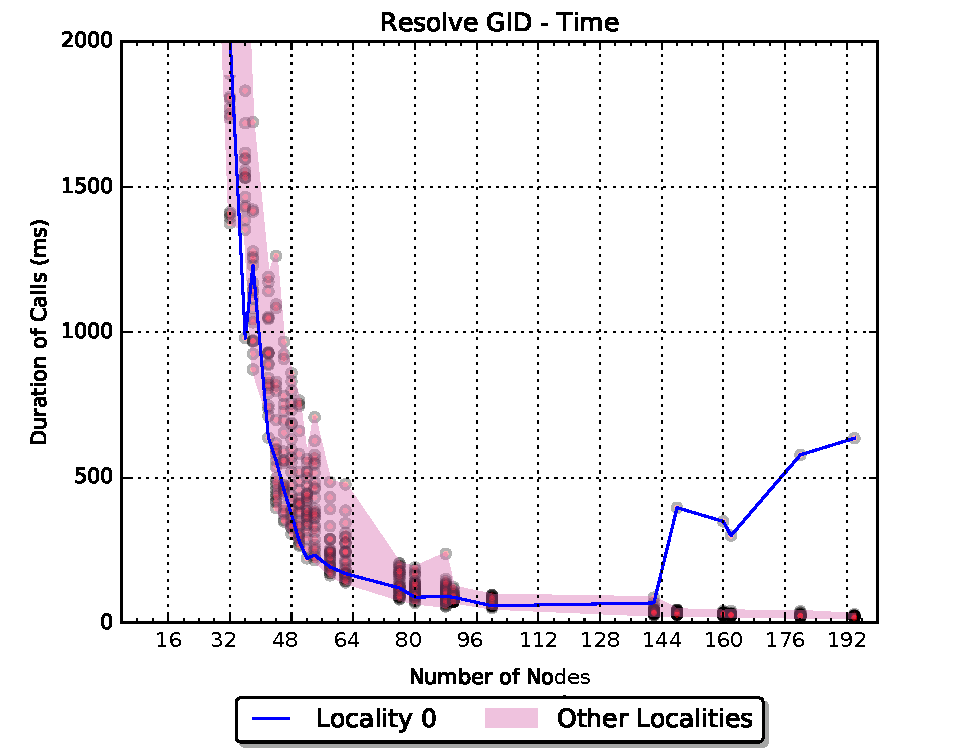
\includegraphics[width=.54\textwidth,height=\textheight,keepaspectratio]{graphs/octotiger_resolve_gid_time}
    \caption{Total time spent to resolve GID calls while running OctoTiger on 32 to 194 nodes of SuperMIC with fixed problem size (Strong Scaling). Each (red) circle refers to the measured amount of time a locality has spent executing resolve GID calls. Higher intensities indicate overlapping measurements. The line highlights locality 0's behavior. X axis starts from 2 to keep consistency with the X axis on other plots.}
    \label{fig:octgr_strong_resolve_gid_time}
\end{figure}

Appropriate distribution of work is of particular interest to computer
scientists. In case of AGAS, ideally we expect the number of specific
operations and the amount of time spent to perform them to be similar. Address
resolution is one of the main functions of AGAS that translates a HPX GID to
the actual virtual address on a machine. Its operation is complicated if the
object is not currently located on the locality that address resolution is taking
place and in such case AGAS tries to determine which locality the object
currently lives on, serialize the task that asked to access the foreign GID in
an HPX parcel, and send it to the locality the object is living in. If an AGAS
instance has no knowledge of the locality that is holding an object then it
takes advantage of the fact that a locality on which an object is created stays
responsible for it during the object's entire lifetime and uses the metadata in
the GID to determine the locality on which the object was originally created and
sends the query there. Fig. \ref{fig:octgr_strong_resolve_gid_time} shows the
amount of time GID resolution takes while running OctoTiger. By looking at
the graph we notice that while the amount of work performed by each
locality is relatively similar up to 146 nodes, locality 0 starts to perform
more work than other localities. This may indicate that most objects globally
referenced were created on locality 0 and it requires further investigation to
determine if this effect is caused by application behavior, non-optimal data
distribution, or HPX itself.
% What else do I say?!

Parcels are the basic communication block in HPX. Parcels are active messages
that trigger an operation on the target AGAS instance that opens them and
usually contains a serialized task and its arguments. Parcel routing is the
operation in which a parcel is sent to a different locality. We expect that localities exchange a similar amount of parcels and thus, spend a similar amount of time. Fig.
\ref{fig:octgr_strong_route_time} shows that locality 0 ends up handling a
disproportionate and increasing number of routing requests regardless of the
change in data access pattern and size due to scaling. Therefore, the routing
operation is a candidate for optimization.

\begin{figure}[t]
    \centering
    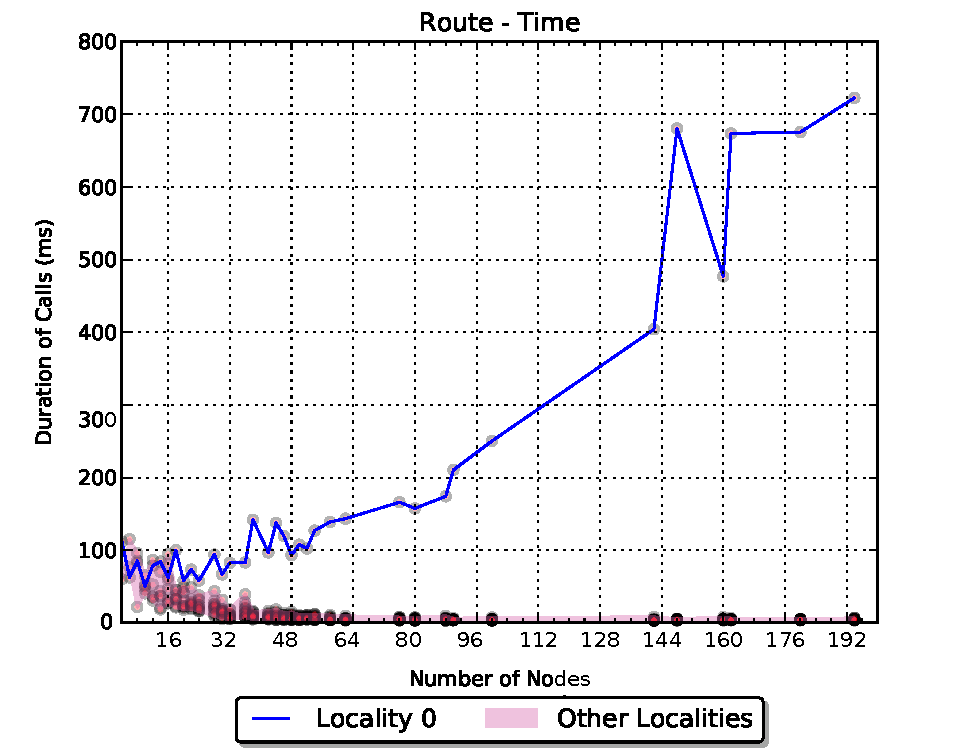
\includegraphics[width=.54\textwidth,height=\textheight,keepaspectratio]{graphs/octotiger_route_time}
    \caption{Total time spent to route calls while running OctoTiger on 2 to 194 nodes of SuperMIC with fixed problem size (Strong Scaling). Each (red) circle refers to the measured amount of time a locality has spent executing parcel route calls. Higher intensities indicate overlapping measurements. The line highlights locality 0's behavior.}
    \label{fig:octgr_strong_route_time}
\end{figure}

% Garbage collection not done much in OctoTiger
For a garbage collection system to function the HPX runtime system must be able
to determine if an object is currently being used. HPX uses reference counting
for local references and a credit-based system to keep track of global
references. The operations that lend and return credits are called decrement
credit and increment credit, respectively.

%One issue that affects our
%experiment is that OctoTiger uses unmanaged objects and therefore AGAS garbage
%collection is not heavily relied upon and therefore the amount of time spent on
%global reference management is not a fair example of applications that do use
%garbage collection.  Despite this limitation, the large number of nodes and the
%limited usage of the operation still enables us to observe the changes in
%decrement credit's behavior as the number of nodes increase.
Fig \ref{fig:octgr_strong_decr_cred} depicts the behavior of \textit{decrement\_credit}
calls that take place while running OctoTiger with the same number of objects as
the number of nodes are increased. This figure shows that a
linear increase in number of objects results in an exponential growth
in the amount of time spent on managing global references. Although this
behavior is likely to be different for applications that do not have as many
global references per each object and therefore \textit{decrement\_credit} is a good
candidate for further optimizations.

\begin{figure}[t]
    \centering
    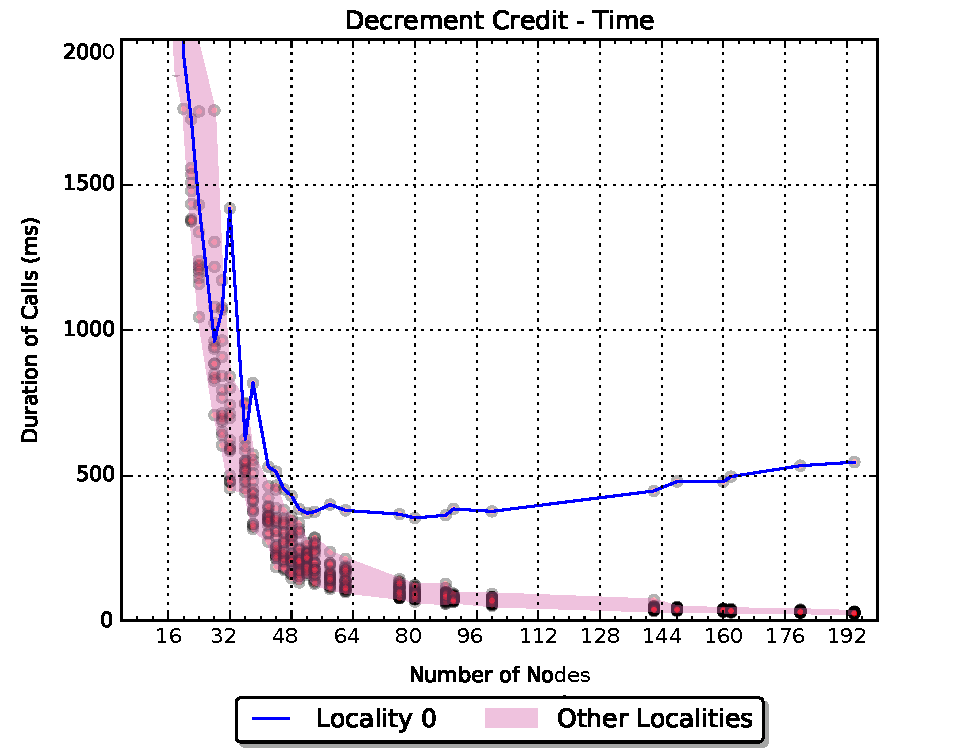
\includegraphics[width=.54\textwidth,height=\textheight,keepaspectratio]{graphs/octotiger_decrement_credit_time}
    \caption{Total time spent to decrement credit calls while running OctoTiger on 2 to 194 nodes of SuperMIC with fixed problem size (Strong Scaling). Each (red) circle refers to the measured amount of time a locality has spent executing resolve GID calls. Higher intensities indicate overlapping measurements. The line highlights locality 0's behavior.}
    \label{fig:octgr_strong_decr_cred}
\end{figure}

% We didn't collect all execution times
% The values are small
Table \ref{tab:exec-percent} shows the percentage of execution time that is
spent on maintaining AGAS and the percentage of execution time that is spent on the three most expensive AGAS operations. It is worth mentioning that we did not plan to
collect execution times for all runs and incidentally collected these
values, but we nevertheless expect the values to be similar for other node
configurations that are not in the table. Based on these values we observe that
AGAS takes only a small amount of execution time.

%\begin{figure}
%    \begin{subfigure}[b]{0.3\textwidth}
%        \centering
%        \caption{Total time spent to resolve GID calls while running OctoTiger on 2 to 194 nodes of SuperMIC with fixed problem size (Strong Scaling)}
%        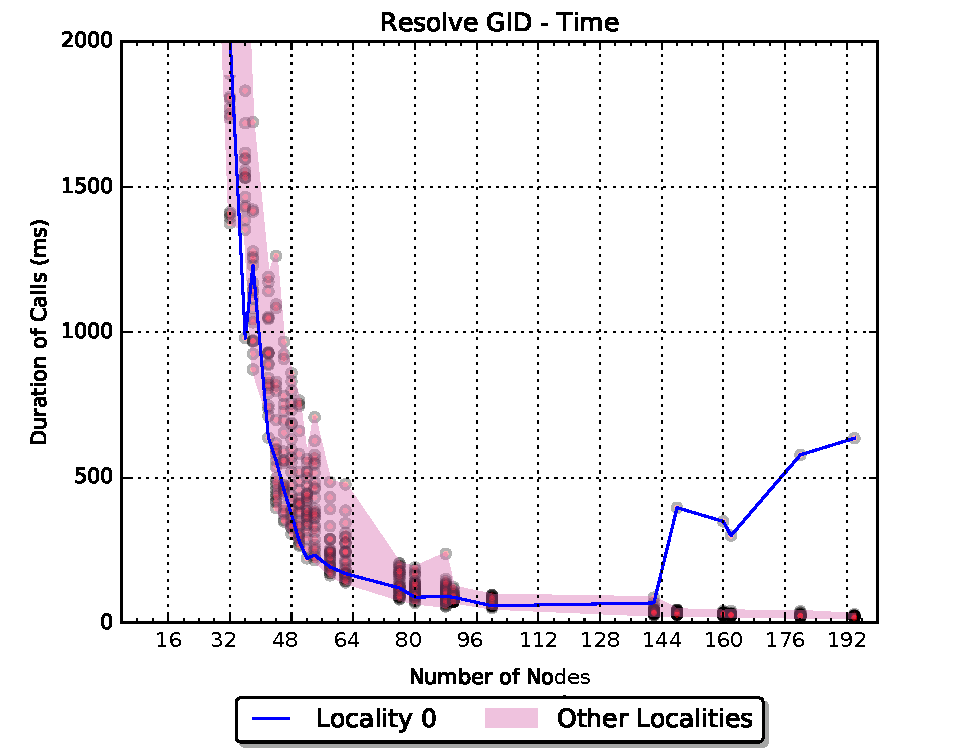
\includegraphics[width=\textwidth,keepaspectratio]{graphs/octotiger_resolve_gid_time}
%        \label{fig:octgr_strong_resolve_gid_time}
%    \end{subfigure}%
%    \hfill
%    \begin{subfigure}[b]{0.3\textwidth}
%        \caption{Total time spent to route calls while running OctoTiger on 2 to 194 nodes of SuperMIC with fixed problem size (Strong Scaling)}
%        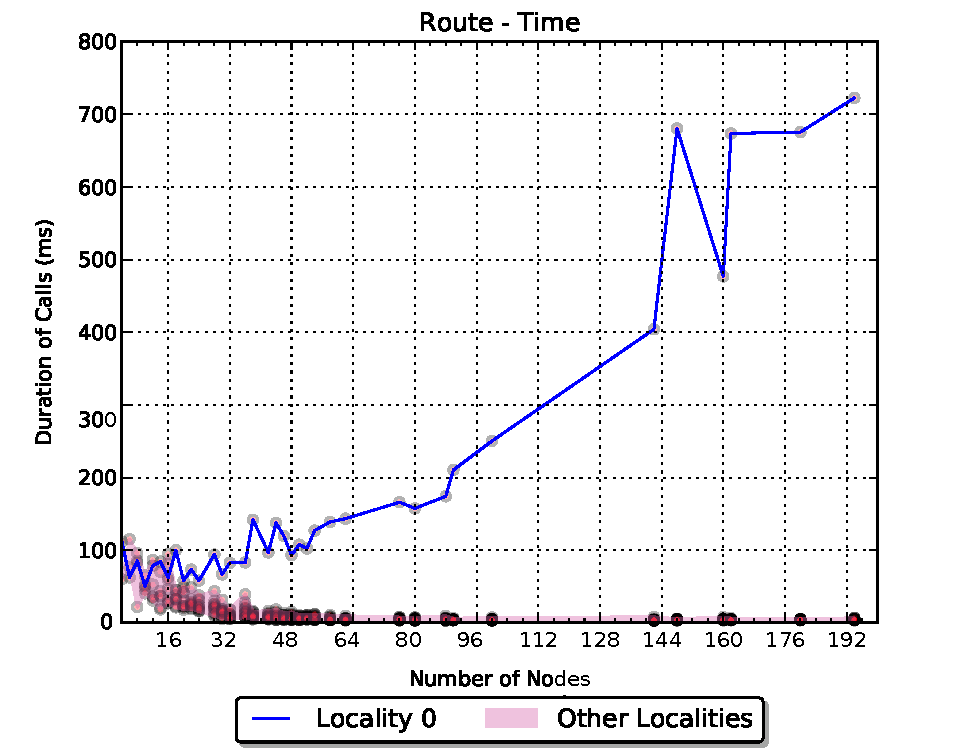
\includegraphics[width=\textwidth,height=\textheight,keepaspectratio]{graphs/octotiger_route_time}
%        \label{fig:octgr_strong_route_time}
%    \end{subfigure}%
%    \hfill
%    \begin{subfigure}[b]{0.3\textwidth}
%        \caption{Total time spent to decrement credit calls while running OctoTiger on 2 to 194 nodes of SuperMIC with fixed problem size (Strong Scaling)}
%        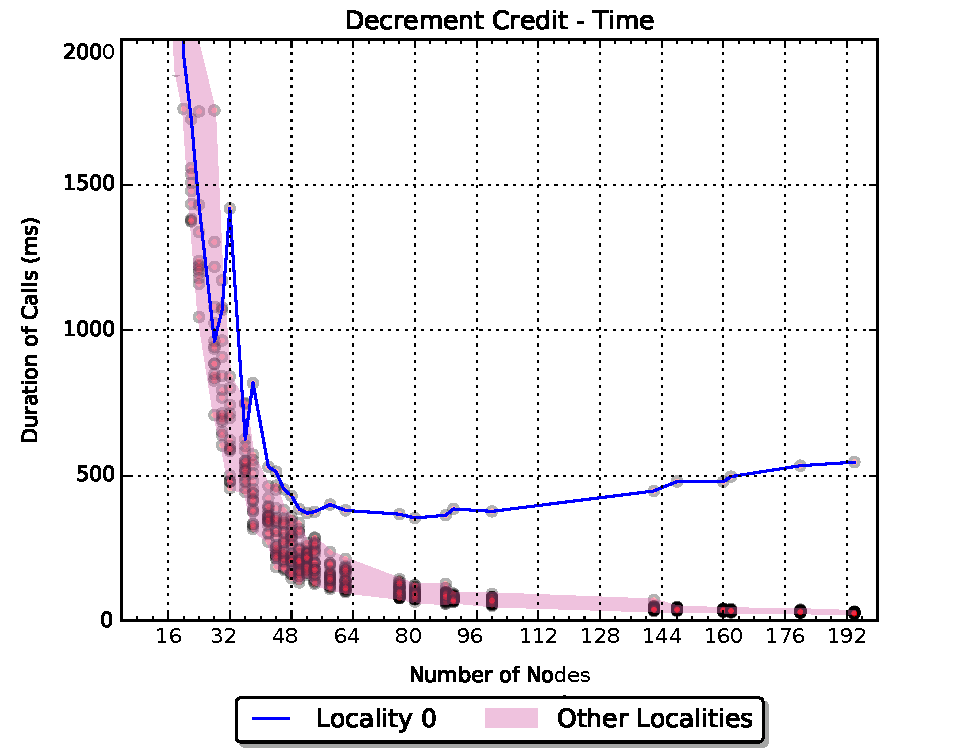
\includegraphics[width=\textwidth,height=\textheight,keepaspectratio]{graphs/octotiger_decrement_credit_time}
%        \label{fig:octgr_strong_decr_cred}
%    \end{subfigure}%
%\end{figure}

